\documentclass[class=report, crop=false, 12pt,a4paper]{standalone}
\usepackage{enumitem}
\usepackage{float}
\usepackage[normalem]{ulem}
\usepackage{graphicx}
\usepackage{amsmath}
\usepackage{amssymb}
\usepackage{siunitx}
\usepackage{commath}
\usepackage{tikz}
\usetikzlibrary{positioning, fit, calc}   
\tikzset{block/.style={draw, thick, text width=3cm ,minimum height=1.3cm, align=center},   
line/.style={-latex}     
}  
\begin{document}
\section{Exercise 2 - Fluid tutorial group B}
A viscous fluid of constant density, $\rho$, and kinematic viscosity, $\nu$, flows over a flat plate inclined at an angle $\alpha$ and moving with a constant velocity $V_w$. The flow is stationary and no pressure gradients are applied. The only body force acting on the fluid is due to gravity, $g$. You can assume zero velocity component in the direction orthogonal to the plate and negligible air resistance at the interface between the viscous fluid and air $(y = h)$.
\subsection{Determine by means of the Navier-Stokes equation the velocity profile, $u(y)$}
NSE (x,y):
\begin{gather}
  \frac{\partial u}{\partial t} + u \frac{\partial u}{\partial x} + v\frac{\partial u}{\partial y} = -\frac{1}{\rho}\frac{\partial p}{\partial x} +\nu \left[ \frac{\partial^2 u}{\partial x^2} +\frac{\partial^2 u}{\partial y^2} \right] + f_x\\
  \frac{\partial v}{\partial t} + u \frac{\partial v}{\partial x} + v\frac{\partial v}{\partial y} = -\frac{1}{\rho} \frac{\partial p}{\partial y} +\nu \left[ \frac{\partial^2 v}{\partial x^2} +\frac{\partial^2 v}{\partial y^2} \right] + f_y
\end{gather}
\begin{itemize}
  \item $\frac{\partial}{\partial t} = 0 $ steady flow
  \item $v=0$ negligible
  \item $\frac{\partial}{\partial x}$ no variation in flow along plate length
\end{itemize}
\begin{align}
  0 + 0 + 0 &= 0 + \nu \frac{\partial^2 u}{\partial y^2} + g\sin{\alpha}\\
  0+0+0 &= -\frac{1}{\rho}\frac{\partial p}{\partial y} -g\cos{\alpha}\\
  \frac{\partial^2 u }{\partial y^2} &= -\frac{g \sin(\alpha)}{\nu} \label{doublediffuy}\\
  \frac{\partial p}{\partial y} &= - \rho g \cos{\alpha}
\end{align}
Integrating equation (\ref{doublediffuy}) once:
\begin{equation}
  \int \left( \frac{\partial^2 u}{\partial y^2} \right) \dif y = \int \left( -\frac{g\sin{\alpha}}{\nu} \right)\dif y \\
  \frac{\partial u}{\partial y} = -\frac{g\sin{\alpha}}{\nu}y + C
\end{equation}
Apply the following boundary equation, due to 0 air resistance at $y=h$ boundary:
\begin{equation}
  \tau(h) = \left. \mu \frac{\partial u}{\partial y} \right|_{y=h} = 0 \\
  \therefore 0 = -\frac{g\sin{\alpha}}{\nu}h + C\\
  C = \frac{g\sin{\alpha}}{\nu}h \label{singlediffuy}
\end{equation}
Integrate equation (\ref{singlediffuy}) once more:
\begin{align}
  \int \left( \frac{\partial u}{\partial y} \right)\dif y &= \int \left( -\frac{g\sin{\alpha}}{\nu}y + \frac{g\sin{\alpha}}{\nu}h \right)\dif y \\
  u(y) &= -\frac{g\sin{\alpha}}{2\nu}y^2 + \frac{g\sin{\alpha}}{\nu}hy + D\\
  y(0) &= -V_w = D\\
  u(y) &= -\frac{g\sin{\alpha}}{2\nu}y^2 + \frac{g\sin{\alpha}}{\nu}hy - V_w\\
  u(y) &= \frac{g\sin{\alpha}}{\nu}y \left(h - \frac{1}{2}y\right) - V_w
\end{align}
\subsection{If the net flow rate across the fluid height is zero, determine the corresponding plate velocity, $V_{wo}$, as a function of $\alpha$}
Volume flow rate:
\begin{align}
  \int_o^h u(y)\dif y &= \int_o^h \left( \frac{g\sin{\alpha}}{\nu} \left(hy - \frac{1}{2}y^2\right) - V_w \right) \dif y\\
  &= \left[ \frac{g\sin{\alpha}}{\nu}y \left(\frac{hy^2}{2} - \frac{1}{6}y^3\right) - V_wy \right]_0^h\\
  &= \frac{g\sin{\alpha} h^3}{3\nu} - V_wh
\end{align}
This is equal to 0 for $V_{wo}$, hence:
\begin{equation}
  V_{wo} = \frac{g\sin{\alpha}h^2}{3\nu}
\end{equation}
\subsection{For the condition found above determine the $y$ coordinate corrsponding to $y=0$. Sketch three velocity profiles for $V_{wo} < V_w $, $V_{w0} = V_w$ and $V_{wo} > V_w$ and comment them}
Combining above equations for $u(y)$, we get:
\begin{equation}
  u(y) = \frac{g\sin{\alpha}}{\nu}y\left(-\frac{1}{2}y^2 + hy - \frac{1}{3}h^2\right)
\end{equation}
Set this equal to 0 and solve:
\begin{align}
  0 &= -\frac{1}{2}y^2 + hy - \frac{1}{3}h^2\\
  y &= \frac{3-\sqrt{3}}{3}\cdot h
\end{align}
\begin{figure}[H]
  \centering
  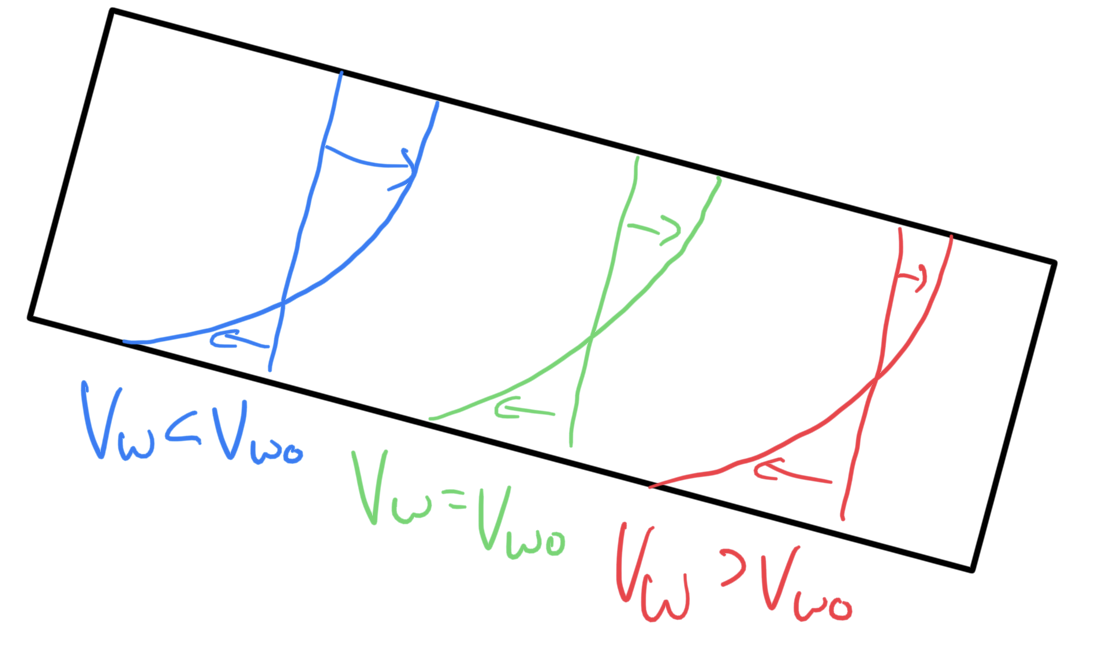
\includegraphics[width = 0.8\textwidth]{../img/velocityprofile004001.png}
  \caption{We can see that in the blue one velocity is increased towards the air boundary. As we move along to the point where $V_w = V_{wo}$, we see that the point where $u=0$ is $\frac{1}{2}h$. Finally we see the velocity highest close to the plate boundary.}
\end{figure}
\subsection{If the flat plate surface is $S$, determine the force, $F$, and power, $P$, required to move it with constant velocity $V_{wo}$}
Using tensor equation:
\begin{equation}
  \tau = \left. \mu \frac{\partial u}{\partial y}\right|_{y=0} = \rho g h \sin{\alpha}
\end{equation}
Power is simply $F \times A \times V$:
\begin{equation}
  P = \tau SV_w = \rho g h \sin{\alpha} SV_w
\end{equation}
\end{document}